\chapter{Development}
In this chapter we will cover the development of all the software employed during the realization of this work, as well as the planning and design of the experiments we desire to make for the benchmarking of both libraries.

\section{Experiment Design}
The first step before starting to record any data or implementing any renderers was to decide what kind of experiments we wanted to run. After reading recent publications on the topic of ray and path tracing, we settled for the same measurements done by Nvidia at the last GTC, when they introduced some advances in real-time path tracing \cite{Clarberg2022}. These are frame time, acceleration structure building time, and memory usage.

\begin{figure}[hbt!]
    \centering
    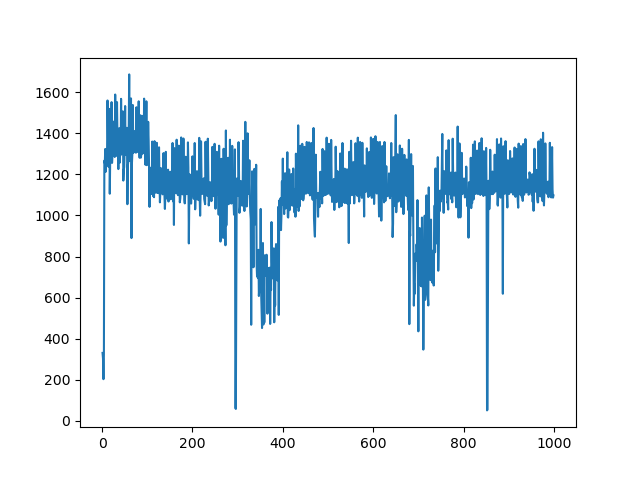
\includegraphics[width=1.0\textwidth]{figuras/vulkan-7680x4320viking_room-textures-frametimes.png}
    \caption{Render times over 1000 frames with a frame buffer resolution of 7680x4320, while drawing the model of a viking room with textures. It can be observed how in a very short span of time, the rendering time of the exact same geometry and effects can hugely change.}
    \label{vulkan-7680x4320viking_room-textures-frametimes}
\end{figure}

\begin{itemize}
    \item[*]\textbf{Acceleration Structure Building Time:} as the name suggests, this is a spatial data structure that speeds up the search for triangles, distance fields and other geometry primitives in a given scene. Ray tracing applications use these to achieve better performance. For example, it's much faster to look for ray intersections by traversing a hierarchical structure of Axis Aligned Bounding Boxes than to check a ray against every triangle in a scene. These structures are typically comprised of a single Top Level Acceleration Structure (TLAS) containing multiple Bottom Level Acceleration Structures (BLAS), which encode a single 3D model each with a 3x4 transformation matrix. These structures are usually implemented in hardware. The time it takes for them to be built can be relevant on the general application's startup time for a static scene such as the ones we will be testing, and for runtime performance in case of scenes with dynamic geometry, where this structure will need to be rebuilt for every animation step.
    \item[*]\textbf{Frame Time:} videogames and the media that traditionally covers them have engraved in the general public the notion that Frames Per Second (FPS) is the most important performance metric in an interactive graphical application. While this is probably true for the end user experience, the FPS count can be affected by a miriad of things outside of the rendering system, such as GPU-CPU synchronization, physics simulation, etc. As this work aims to compare only the rendering performance of each library, we will only be measuring the time it takes to write the rendered images to a frame buffer. Due to the huge variance of running times inside a modern Operating System, the render times can vary wildly as well (as we can see in \ref{vulkan-7680x4320viking_room-textures-frametimes}). To mitigate this, we will take the time measurements over a fairly long period of time (1000 frames) and average them together in order to get a more precise idea of the rendering time that's less subject to flukes.
    \item[*]\textbf{Memory Usage:} quite self-explanatory, the last factor we consider of great importance is the video memory consumption of the process. This can be a limiting factor on the hardware requirements of a particular application, since execeding the user's GPU's memory capabilities will force it to resort to the use of swap memory from the system RAM, significantly impacting the performance due to an abundance of copying between the two.
\end{itemize}

All these variables will be tested while rendering different ammounts of geometry and scene complexity. In order to simplify the development of all renderers, each scene will be comprised of a single 3D model. The Single Triangle model was built in-house, the Viking Room was obtained from \cite{VulkanTutorial}, and the rest were obtained from Morgan McGuire's Computer Graphics Archive \cite{McGuire2022Data}. They all can be seen at table \ref{scenes-geometry-table}

\begin{center}
  \begin{tabular}{ | m{3cm} | m{3cm}| m{3cm}|m{3cm} |}
  \hline
  Model name& Triangles& Vertices& Texture size\\
  \hline
    Single Triangle& 1& 3& 0\\
  \hline
    Viking Room& 2000& 2600& 0\\
  \hline
    BMW& 385079& 249772& 0\\
  \hline
    Sponza& 262267& 184330& 74.0 MB\\
  \hline
    Hairball& 2880000& 1441098&0\\
  \label{scenes-geometry-table}
\end{tabular}
  % \caption{Scenes that will be used to test the ray tracing libraries compared in this work. We have selected a single 3D model from each order of magnitude in terms of size.}
\end{center}

In order to better gauge how these scene sizes compare, we have plotted them in graph \ref{scenes-geometry-graph}.

\begin{figure}[hbt!]
  \centering
  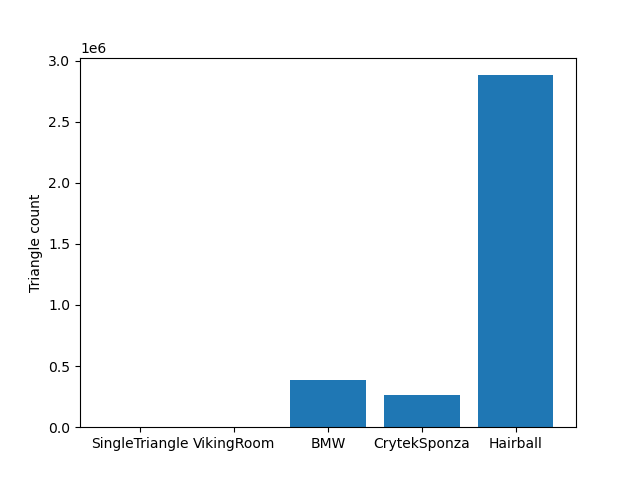
\includegraphics[width=0.75\textwidth]{figuras/scenes-geometry.png}
  \caption{Triangle count of each scene used to test both renderers. We can see how there are orders of magnitude of difference every two of them.}
  \label{scenes-geometry-graph}
\end{figure}

After testing these models we countered some discrepancies with the Acceleration Structure Build Times we expected for each of them. This can be seen in more detail in the Results chapter. We added some extra models for further testing. Their features can be seen in table \ref{extra-scenes-geometry-table} and their triangle counts is graphically compared in plot \ref{extra-scenes-geometry-graph}

\begin{center}
  \begin{tabular}{ | m{3cm} | m{3cm}| m{3cm}|m{3cm} |}
  \hline
  Model name& Triangles& Vertices& Texture size\\
  \hline
    Human& 25422& 29708& 0\\
  \hline
    ISCV2& 383511& 193212& 0\\
  \hline
    Gallery& 998831& 499314& 0\\
  \label{extra-scenes-geometry-table}
\end{tabular}
  % \caption{Scenes that will be used to test the ray tracing libraries compared in this work. We have selected a single 3D model from each order of magnitude in terms of size.}
\end{center}

\begin{figure}[hbt!]
  \centering
  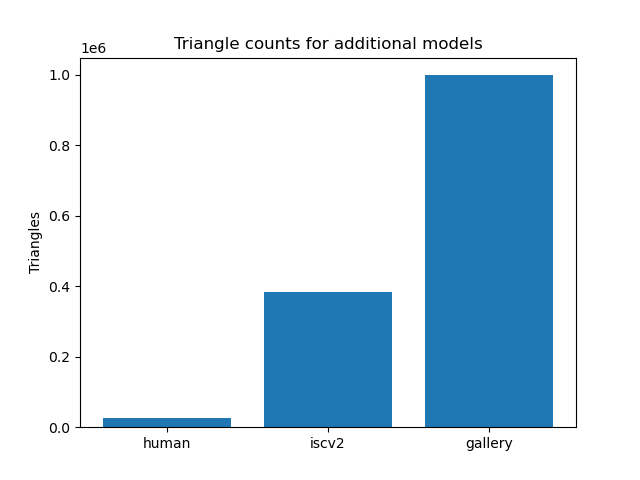
\includegraphics[width=0.75\textwidth]{figuras/extra-scenes-geometry.png}
  \caption{Triangle count of the extra scenes used to further test acceleration structure build times.}
  \label{extra-scenes-geometry-graph}
\end{figure}

Finally, we considered it will be of use compare how each library performed in different hardware configurations. We gathered all the available hardware compatible with GPU accelerated ray tracing, and used it to run the same experiments. This hardware is summarized in table \ref{pc-specs-table}. This will not only allow us to check how different GPUs handle the same workload, but also how they do it inside a virtualized environment: the Intel Core i9 machine is not running the software in bare metal, but rather virtualizing Windows under \textit{QEMU}.

\begin{center}
  \begin{tabular}{ | m{5cm} | m{3.5cm}| m{2cm}|m{4cm} |}
  \hline
  CPU& GPU& RAM& OS\\
  \hline
    Intel Core i7-12700K, 3.60 GHz& Nvidia GeForce RTX 3070& 16 GB& Windows 11, 64 bit\\ % Paco
  \hline
    AMD Ryzen 5 3600 3.6GHz BOX& Nvidia GeForce RTX 2070 Super& 16 GB& Windows 10, 64 bit\\ % Mine
  \hline
    Intel Core i5-9600K, 3.7GHz& Nvidia GeForce RTX 3060 Ti& 16 GB& Windows 10, 64 bit\\ % Juan Carlos
  \hline
    Intel Core i9-9900K (12/16 cores), 3.6GHz& Nvidia GeForce RTX 3080& 16 GB& Windows 10, 64 bit\\ % Roobre
  \hline
    Intel Core i7 10th gen& Nvidia GeForce RTX 3080& 32GB& Windows 10, 64 bit\\ % Naru
  \label{pc-specs-table}
\end{tabular}
  % \caption{Hardware information of the different PCs we managed to run our tests on.}
\end{center}

\clearpage


\section{Implementation}
In this section we will discuss the process of implementing everything that went into this work. The code written for this comparison can be divided in three categories:

\begin{itemize}
    \item[*]{Two different renderers with as close as function parity as we could, and relying in the same third party libraries for interacting with the operating system and file I/O.}
    \item[*]{A series of scripts to automate testing and write performance data to disk.}
    \item[*]{A system for generating the plots and graphs in this work from the performance data generated.}
\end{itemize}

In both renderers we used \textit{TinyObjLoader} and \textit{stb\_image} for loading 3D models in \textit{.obj} format and \textit{GLFW} for handling the window and user input. The phases of loading models and presenting the rendered image to the screen are out of the scope of this work, so they will be left out of every measure we do. As such, we do not measure the time for loading models and presenting an image to the screen.

\subsection{OptiX Renderer}
First developed by Nvidia around 2009, this ray tracing API allows to offload computations to one or multiple Nvidia GPUs using their own technology CUDA. It has been used in other applications aside from computer graphics where line-of-sight is important, namely optical and accoustical design, radiation and electromagnetic research, artificial intelligence queries and collision analysis. This API is heavily documented in their programming guide, and several beginner-level tutorials have been made for it.

We took the course from \textit{SIGGRAPH 2019/2020} by Ingo Wald in which you learn how to build a simple 3D model viewer capable of simple lighting. Our resulting renderer is very much a typical one consisting of:

\begin{itemize}
  \item[*]{A Ray Generation program on device (GPU) that computes pixel colors. This is called from CUDA, although it requires a "launch parameters" \textit{struct} to be both in device and host (CPU) memory. This structure will encode things like the camera data and acceleration structure (AS). It allows for compaction in the AS, but we will not be diving in it's implementation details here. The program will also need sub-programs for when a ray either misses or hits scene geometry. This CUDA code is compiled and embedded into the C++ host code during compilation.}
  \item[*]{A pipeline, which will handle the kind of programs that we want to run. For this we will need to create an OptiX Context and Module with the embedded CUDA code and set up the required program groups that will go into such pipeline (raygen, miss, hit group). Finally, with all this information we can initialize an OptiX Pipeline.}
  \item[*]{A Shader Binding Table (SBT), which will handle the exact configuration for the programs we will be running. It's a set of "ray generation", "miss" and "hit group" records to run. Each record contains a header describing the program to run and user-supplied data, like per-mesh CUDA texture objects. All these records are filled during creation of the SBT and need to be uploaded to a CUDA buffer.}
  \item[*]{A Frame Buffer in which to store the generated image. After measuring the rendering time, we copied the buffer's contents to a GLFW window using OpenGL. This allowed us to get immediate feedback on what the renderer was doing.}
\end{itemize}

In order to add hard shadows to the scene, we implemented a new ray type with it's own "closest hit" and "any hit" programs (in this case all the work happens in the "any hit" one, with the others doing nothing for shadows). To keep the development time reasonable we assume all surfaces are opaque, killing the ray upon it's first occlusion. As a result of this second ray type, the Hitgroup Program Group has two entries (one for radiance rays and one for shadow rays) and the SBT has to create two records per mesh. In our case we use the same data in both records, although this is not mandatory.

Finally we ported the resulting code from OptiX 7.3 to 7.5, it's latest version. This required only a couple of minimal changes.

From that starting point we instrumented the ported code in order to measure frame rendering time, acceleration structure building time and memory consumption, as well as parametrizing values for frame buffer width and height and which 3D model to load. We used the \textit{chrono} library from the C++ STL and it's \textit{high\_resolution\_clock} for measuring time and the function \textit{cudaMemGetInfo()} to consult the memory usage. We built all this functionality in a class \textit{FramePerformanceCounter} that handled data recording and file I/O, making it easy to share this functionality between renderers.

\subsection{Vulkan Renderer}
First announced by the Khronos Group at GDC 2015 as the "next generation OpenGL", Vulkan is intended to be used in high-performance real-time 3D graphics for interactive applications such as videogames, offering higher performance and lower level control than popular graphics APIs at the time such as OpenGL or DirectX 11.

It employs an extension system in which the programmer must explicitly ask for the functionality they require, therefore reducing unnecesary overhead and code size. It is through this system that it provides ray tracing support, by means of the \textit{VK\_KHR\_ray\_tracing} extension, while usually focusing on traditionally rasterized graphics.

This phase was the lengthiest of the whole development process. Vulkan, highly explicit, requiring the programmer to recreate the whole rendering pipeline and configure every stage for drawing even the simplest scenes. The following steps require significantly less effort, though it does not decrease as greatly as it does with OptiX.

\subsubsection{Rasterized}
We started by building a traditional rasterized renderer based on the one from the Vulkan Tutorial \cite{VulkanTutorial}, which allowed us to get familiar with the API before using it for tracing rays, as well as giving us the opportunity of comparing ray traced graphics to rasterized ones with as similar features as possible. We then instrumented and parametrized it almost as we did with the OptiX renderer. The main difference was querying for memory usage using the \textit{DirectX Graphics Infrastructure} API \cite{DXGI} as explained in \textit{There is a way to query GPU memory usage in Vulkan - use DXGI} \cite{GpuMemUsageVulkan}. Even though we could have used the Vulkan extension \textit{VK\_EXT\_memory\_budget}, we decided against it since it was harder to figure out it's usage compared to the more straight forward \textit{DXGI}.

\subsubsection{Ray Traced}
We expanded our rasterized Vulkan renderer following the course by Nvidia on this very topic \cite{VulkanRaytracingTutorial}, which gave us a simple ray tracer capable of rendering 3D models and adding some lights. On a high level, this renderer has similar components to the one we wrote in OptiX, with some differences:

\begin{itemize}
  \item[*]{Acceleration Structure (AS). As with the rasterized renderer, Vulkan is much more explicit than even the relatively low-level OptiX 7, making us manually convert our triangle geometry data into multiple structures that will be consumed by an AS Builder. This builder will then store it in one or multiple Bottom Level Acceleration Structures (BLAS). As with the OptiX raytracer, we indicate (to the AS Builder this time) that all our geometry is opaque, disabling calls to the "anyhit" shader. Each BLAS also allows for compaction. Broadly speaking, it works by querying the initial (large) BLAS for only the values we require, creating a new BLAS with a smaller size, copying the data we have to the newly allocated one and destroying the large BLAS. It requires waiting until a whole BLAS is built since only then we know how much memory it actually uses.

With these BLASes we build a single Top Level Acceleration Structure (TLAS). This is the entry point for the ray tracing scene descriptor, as we will explain later, and stores all the geometry instances. Each instance is represented by a transform matrix, a BLAS ID, an instance ID and a "hit group" index. This index represents the shaders that will be invoked uppon hitting the stored object, and are tied to the definition of the Shader Binding Table and the Raytracing Pipeline, as we shall see. Since our renderer only uses one hit group, this index will always be 0. Once all the configuring is done, we build the TLAS. We have decided to optimize for ray tracing performance instead of memory size, though this option doesn't seem to be present in OptiX.}

  \item[*] {Ray Tracing Descriptor Set. This component references external resources used by shaders. In the rasterized graphics pipeline we can group the rendering objects by the materials they use, and draw all the objects that use some materials all together. This way, we only need to bind the descriptor set that references those materials while rendering the objects they use them. In Ray Tracing, however, we can't know which objects in the scene will be hit by a ray, and as such any shader can be invvoked at any time. Thus, we need to use a set of Descriptor Sets containing all the resources necessary to draw the scene (like all the textures of all the materials). Finally, since the Acceleration Structure contains only position data, the geometry's vertex and index buffers need to be passed to the shaders so that they can manually look up the rest of the vertex attributes.}
  \item[*]{Ray Tracing Pipeline. As mentioned earlier, we need to have every shader available for execution at any time when raytracing, and the shaders to execute are selected on the GPU at runtime. The structure that makes this selection possible is a Shader Binding Table. This is essentially a table of opaque shader handles (probably device addresses) analogous to a C++ v-table. As with everything in Vulkan, we have to build this table ourselves. A high level overview of this process is:
    \begin{enumerate}
      \item Load and compile shaders into \textit{VkShaderModule}s in the usual way.
      \item Package said \textit{VkShaderModule}s into an array of \textit{VkPipelineShaderStageCreateInfo}.
      \item Create an array of \textit{VkRayTracingShaderGroupCreateInfoKHR}. Each element will eventually become an SBT entry. At this point, each shader group references a single shader by it's index in the array created created in the last step.
      \item Compile the two arrays created plus a pipeline layout (as usual) into a ray tracing pipeline. This converts the array of shader indices into an array of shader \textit{handles}. We can query this at will.
      \item Allocate a buffer for the SBT and copy the handles to it.
    \end{enumerate}
    The ray tracing pipeline is more similar to the compute pipeline than the rasterization pipeline: ray traces are dispatched in an abstract 3D space, with it's results manually written using \textit{imageStore}. However, unlike the compute pipeline, we dispatch individual shader invocations, rather than local groups.

    The entry point for ray tracing is the ray generation shader, which we call for each pixel. It typically initializes a ray starting at the location of the camera in the direction of the camera lens model at it's corresponding pixel's location. The miss shader and a closest hit shader, which work in the same way as in OptiX.

    The \textit{intersection} shader is used to intersect user-defined geometry. This can be useful for intersecting placeholders when using on-demand geometry loading, or procedural geometry without tessellating it beforehand. We will not be using this type of shader in this work, since it requires modifying how the acceleration structures are built. Instead, we will solely use the ray-triangle intersection test provided by the Vulkan extension, which returns 2 floats representing the barycentric coordinates of the hit point inside a given triangle.

    Finally, the \textit{any hit} shader is executed in each potential intersection. When we look for the closest hit point to the ray origin, we may find several candidates. The any hit shader is often used to efficiently implement alpha testing so we know if the ray traversal can continue. The default any hit shader is a simple passthrough that returns the intersection to the traversal engine, which determines which intersection is the closest. We will not be using this shader during this work as all our geometry is opaque.}
  \item[*]{As mentioned before, the Shader Binding Table (SBT) works as the blueprint of the ray tracing process. It helps selecting the shaders to use as an entry point, in case of rays missing geometry, and which hit shader groups can be executed for each geometry instance. The link between instances and shader groups is created when setting up the geometry, as we provided a hit group ID in the TLAS for each instance. This value is used to calculate the SBT index corresponding to the hit group of said instance.

    From an implementation standpoint, the SBT is just 4 arrays containing the handles of the shader groups used in the ray tracing pipeline. There is one array for each shader group, namely ray generation, miss, hit and callable (not used in this work). Since we only have one shader of each type, for us each "array" is just a handle to a group of shaders.}
\end{itemize}

We employed the \textit{nvvk} utilities at the \textit{Nvpro} library \cite{Nvpro} to facilitate building this renderer. The same instrumentation and parametrization as in the rasterized renderer was used here.

\subsection{Automation and Plotting}
To get reproducible results in a reduced ammount of time, we implemented a series of Python scripts in order to run every renderer with every combination of scenes, renderer settings (like use of shadows or textures) and framebuffer resolutions. Each renderer run will handle savingtheir performance information to disk. We later plotted these results in a single script using \textit{matplotlib} to more easily gauge how each library behaved under the same configuration. The whole suite of experiments ran just under 10 minutes in every machine we tested it on.
